% !TeX root = ./00.ppgcc-2020.tex

\chapter{Proposta e Metodologia}\label{cha:proposta}

% % Uma Implementação paralela do algoritmo de Detecção de Novidade em Streams MINAS

% A Internet das Coisas (\iot) é composta por vastas quantidades de dispositivos
% conectados à Internet e distribuídos geograficamente.
% Com capacidades diversas providas por elementos como sensores e atuadores, esses
% dispositivos produzem e consomem Fluxos Contínuos de Dados (\streams) com
% diversos objetivos.
% Alguns cenários de \iot envolvem a mineração desses fluxos (\streamMining) em busca de
% padrões para tomada de decisão e, por vezes requerem também baixa latência.
% Para casos de baixa latência ou alta vazão, conexões adequadas para
% processamento em nuvem nem sempre são possíveis ou desejáveis; para esses casos,
% a computação em névoa (\fog) é uma solução.

% O tema de \streamMining envolve a classificação de novos elementos,
% que podem tanto estar relacionados aos dados ou aos metadados das comunicações,
% com base em um modelo.
% \hlke{Porém, como \streams variam temporalmente e são ilimitados,}
% as classes contidas em um \stream não são todas previamente conhecidas.
% A identificação e classificação de novas classes em \streams é denominada
% Detecção de Novidades (\novelty, \nd) em \streams.

% % \hlfa{Além dos aspectos}
% % \notafa{rever o parágrafo. Varios conceitos errados... a identificação de novas
% % classes é denominada detecção de novidade.... data stream variam temporalmente}
% % inerentes a \streamMining, são considerados na construção de um
% % \hlhl{sistema}
% % \notahl{Poderia reescrever a frase, evitando inversões na estrutura
% % sujeito/verbo e complementos. Yoda!}
% % que computa \streams a taxa de eventos
% % % (itens atômicos de um \stream)
% % gerados por cada produtor e o número de produtores nesse sistema, totalizando o
% % volume de eventos 
% % \notahl{qual sistema?}
% % \hlhl{do sistema}.
% % % Além do volume de eventos é necessário
% % Volumes elevados dificilmente são computados em apenas um nó (e muito menos em
% % um único núcleo processador) e por isso, esses sistemas \hlhl{geralmente} são distribuídos.

% Sistemas que utilizam \nd para \streams gerados por dispositivos \iot devem
% utilizar algoritmos que considerem os desafios inerentes a fluxos de dados
% (\evolution e \drift) para adequada detecção de novidades e, para tanto,
% requerem processamento em arquiteturas
% que atendam os requisitos de volume de mensagens e latência de detecção.
% O algoritmo MINAS é adequado para esse caso, pois trata os desafios de
% \streamMining, porém não tem ainda implementação que atenda os requisitos de
% volume e latência, especialmente para aplicações \iot onde um ambiente de \fog é
% atrativo.

% % \notahl{Com relação à proposta, será que é o caso de indicar que a
% % arquitetura apresentada é uma proposta inicial, que será refinada ao longo da
% % pesquisa?}

% Para preencher a lacuna de algoritmo de \nd em ambiente \fog, propõem-se então
% o \mfog, uma implementação distribuída do algoritmo MINAS 
% %sobre a plataforma \flink, que
% considerando  um ambiente de \fog.
% O \mfog descrito neste documento foi refinado com os resultados dos experimentos
% descritos na \refsec{resultados}. 
% % e poderá ser revisado ao longo da pesquisa conforme os resultados de outros experimentos evidenciarem obstáculos ou oportunidades de melhoria.

% % \nota{Reestruturar:
% %   A - remember,
% %   B - cenário (iot, fog, stream),
% %   C - problema (4.1, ND em fog, terminar com minas e cassales),
% %   D - solução (4.2, apresetnação, resumo \mfog, metodologia)
% % }
% % \nota{Falta: fog, processamento distribuído de streams, detecção de novidade}


% Este Capítulo apresenta a proposta deste trabalho e a metodologia estabelecida
% para atingir os objetivos.
Neste trabalho investiga-se uma arquitetura e implementação adequada para
executar \acf{ND-DS} em ambiente de névoa para detecção de intrusão em redes de
dispositivos \acf{IoT}.
% In this work, we investigate an appropriate architecture for performing \nd at
% the edge, as a means of allowing small IoT devices to filter and detect undesirable
% network behavior.
Esta abordagem é baseada na arquitetura \arch \cite{Cassales2019a} e no algoritmo
de \nd \minas \cite{Faria2016minas}.
% Our approach is based on the \arch architecture \cite{Cassales2019a} and \nd
% techniques provide by the \minas algorithm \cite{Faria2016minas}.
Nomeada \mfog, esta implementação do algoritmo \minas explora computação distribuída
habilitando o uso de computadores de baixa potência e recursos limitados presentes no
ambiente de névoa a realizar, além de tarefas habituais de um \emph{gateway} \iot, a classificação e detecção de
tráfego indesejável.
% Named \mfog, our distributed algorithm explores load balancing to enable low
% profile devices at the edge of the internet to also work on the classification
% and detection of unwanted traffic.

A arquitetura física do \mfog pode ser vista na Figura
\ref{fig:arq-fisica-mfog}, onde um dispositivo \emph{gateway} observa o tráfego da rede local (sensores IoT) e entre a rede local e 
a nuvem. A detecção de intrusão é executada de forma paralela e distribuída numa névoa de 
dispositivos SBC (\emph{Single Board Computer}). 

\begin{figure}[htb]
  \centerline{
    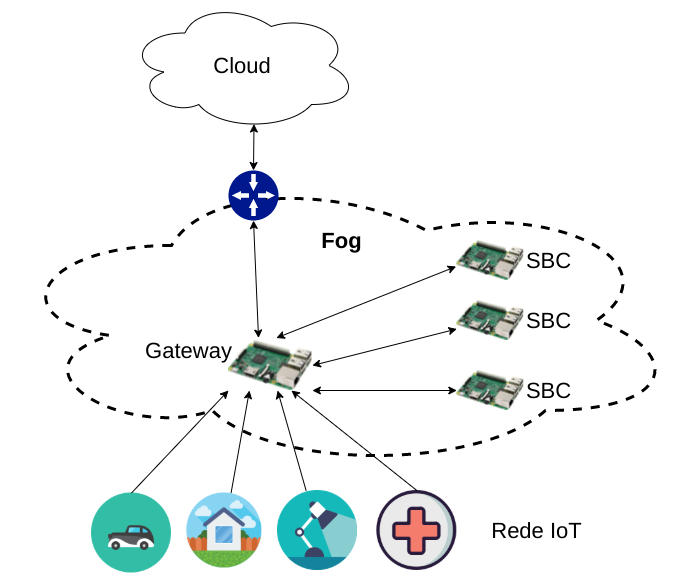
\includegraphics[width=0.6\linewidth,page=1]{figures/arq-mfog.png}
  }
  \caption{Arquitetura física do \mfog.}
  \label{fig:arq-fisica-mfog}
\end{figure}


\acf{NIDS} monitoram o tráfego em redes e analisam as características de cada
fluxo de rede com objetivo de identificar intrusos e tráfegos indesejados.
% monitor network traffic, and analyze the characteristics of each flow 
% to identify any intrusion or misbehavior.
No entanto, este problema requer respostas rápidas e acuradas \cite{DaCosta2019a}:
rapidez é necessária para executar uma ação adequada antes que
maior dano seja feito à rede, e para lidar com a velocidade do tráfego sem impor
atraso ou perda de pacotes na rede observada;
% However, this problem requires both fast and accurate response 
% fast response is needed to have a proper reaction before harm can be cast
% to the network and to cope with the traffic without imposing loss or delay
% in the \nids or observed network;
acurácia é necessária para não  identificar padrões incorretamente, gerando falso
alarme ou ignorando ataques.
% accurate response is required as not to misidentify,
% especially the case of false positive that leads to false alarms.
% To achieve those goals, we leverage fog computing.

% In this work, we propose and assess \mfog, a distributed data stream
% novelty detection system based on the algorithm \minas for securing \iot networks.
% \mfog implements a distributed version of \minas according to the \arch
% architecture proposed in a previous work \cite{Cassales2019a}, to execute in the
% edge where small devices and constrained resources may be prevalent.

Em cenários \iot comuns, dados são capturados por pequenos dispositivos
computacionais e enviados para a nuvem (\cloud) se mais mais recursos
computacionais ou de armazenamento são necessários. Contudo, para \nids e o
requisito de resposta rápida, esta abordagem pode não ser viável. 
Para atender a essa necessidade a Computação em Névoa é uma alternativa promissora.
% In common \iot scenarios, data is captured by small devices and sent to the
% cloud for any compute or storage tasks, but this is not feasible in a \nids
% scenario.

A infraestrutura de Computação em Névoa (\fog) oferece capacidades de realocar
parte do processamento e armazenamento dos provedores de nuvem, posicionando
dispositivos de capacidade intermediária próximos aos usuários e às fontes de dados.
% Fog computing infrastructure aims to offload processing from the cloud
% providers by placing edge devices closer to end-users and/or data sources.
% Para atingir estes objetivos, a presente proposta utiliza computação distribuída
% em névoa, permitindo processamento escalável e mais próximo da rede \iot.
Dada a natureza distribuída e o típico uso de pequenos computadores em cenários
de \iot e névoa, alguns desafios para implementação \nids são notáveis:
% However, given the distributed nature and the typical use of small computing
% devices in IoT scenarios, new challenges arise:
\begin{enumerate}[label=(\emph{\roman*})]

  \item O tráfego nas bordas da rede é inerentemente distribuído, sem uma
  entidade centralizadora que tenha acesso a todas as transmissões;
  
  \item A tarefa de classificação do algoritmo deve ocorrer em paralelo em
  diferentes nós;
  
  \item A tarefa de detecção de novidade, que provê a atualização do modelo,
  deve ser assíncrona;
    
  \item A complexidade do algoritmo (tempo e espaço) deve permitir sua execução em
  computadores modestos, isto é, pouca memória ($< 1GB$) e processadores de
  pouco desempenho.

\end{enumerate}

Nesta proposta, recursos em névoa são combinados para minimizar a latência entre
o recebimento (ingestão) do descritor de fluxo e a identificação daquele fluxo.
Executa-se múltiplas instâncias da tarefa de classificação do algoritmo \minas.
% In our proposal, fog and cloud computing resources are combined to minimize
% the time elapsed between a flow descriptor ingestion and intrusion alarm,
% performing the classification step of \minas running multiple
% classifier instances.
Após identificado o rótulo do descritor de fluxo (exemplo), este par (rótulo, exemplo) pode ser
utilizado imediatamente para tomada de decisões e, se o exemplo é rotulado como
``desconhecido'', ele é armazenado para posterior execução assíncrona da tarefa
de detecção de novidade, portanto sem interromper o processo de identificação.
% After the initial classification, the resulting label can be used immediately,
% but if the sample is labeled as \emph{unknown}, this sample must be stored and
% the novelty detection step will be triggered.

Além do multiprocessamento da tarefa de classificação e da execução assíncrona da
tarefa de detecção de novidade na fase \emph{online}, outra mudança em relação
ao \minas original é a remoção do mecanismo de esquecimento de padrões antigos.
Esta remoção tem por finalidade simplificar a atualização e o compartilhamento
do modelo entre as múltiplas instâncias e \emph{threads} concorrentes.
% 
O impacto desta alteração não é grande, pois o algoritmo \minas não estabelece a remoção
permanente dos \mclusters com pouco uso. Essa alteração aumenta marginalmente 
a complexidade computacional da classificação, pois inclui na busca  os padrões menos utilizados.

Já a fase \emph{offline} e a função de detecção de novidades do algoritmo \minas
permanecem as mesmas.

% To have a better overview of our proposal and how it integrates with existing
% \iot environments, Figure \ref{fig:mfog-phy-arch-cloud} depicts such scenario
% showing from bottom to top:
% \iot devices directly connected to a (local) gateway network;
% this gateway network could be as simple as a single Internet router 
% or be more complex by connecting to private clouds or 
% containing more devices providing fog computing capabilities;
% lastly, available over the internet, the traditional public cloud provides
% inexpensive computing and storage on demand.
% In this scenario, the further apart resources are, the more network
% resources need to be employed, and, as with any networked system, the
% higher is the latency.

% \begin{figure}[hb]
%   \centering
%   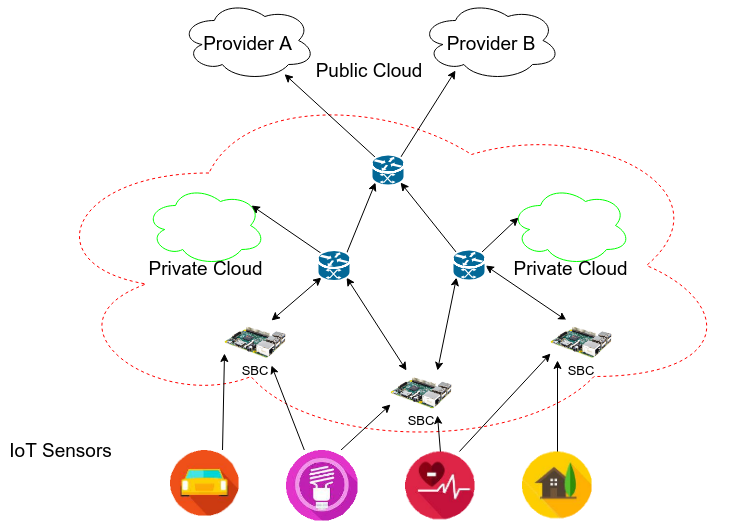
\includegraphics[width=0.5\linewidth]{figures/cassalesimgs-000.png}
%   \caption{\arch \cite{Cassales2019a} physical architecture and deployment scenario overview.}
%   \label{fig:mfog-phy-arch-cloud}
% \end{figure}

A arquitetura geral do \mfog é dividida em dois módulos, Classificação e
Detecção de Novidade, que equivalem à fase \emph{online} do algoritmo \minas.
% The overall \mfog architecture has two main modules, Classification and Novelty
% Detection, which implement the \minas main tasks.
O módulo Classificação executa a tarefa de mesmo nome do algoritmo \minas e é
ponto focal dos esforços de paralelismo desta proposta.
Este módulo é replicado em todos os nós do cluster % hospedado (?)
em névoa.
% The Classification Module performs the same task of the \minas Online phase and
% is the focal point for parallelism and distribution in our proposal.
% It is replicated in the fog and runs on each cluster node, using a configurable
% number of threads (limited to the node CPU core count).

% o que quer dizer isso?
O módulo Detecção de Novidade tem uma instância por cluster, equivalendo a uma
instância por rede local. O compartilhamento de modelo entre
redes distintas é possível, mas não foi implementado e testado neste trabalho.
% 
Este módulo é responsável pela tarefa homônima do algoritmo \minas, recebendo
exemplos com rótulo ``desconhecido'' e os armazenando no conjunto de
desconhecidos; quando o tamanho deste conjunto alcança um valor parametrizado,
este módulo executa a função de detecção de novidade do algoritmo \minas.
% The Novelty Detection Module can also be replicated,
% the choice being one instance per local network, one global cloud instance,
% or both.
% This module also handles the homonymous task of \minas Online phase, receiving
% all the samples labeled with \emph{unknown}, storing them in an internal
% \emph{unknown-buffer}, and, when this buffer is full, performing the \minas
% Novelty Detection task (clustering followed by validation).

\section{Políticas}\label{sec:polices}

O projeto desta arquitetura de \nd distribuída inclui o particionamento das
funcionalidades de \minas e o estabelecimento dos fluxos de dados apropriados
entre os diferentes atores.
 % ??? Hélio
Mudanças no posicionamento de cada ator e no comportamento tem impactos
diferentes no desempenho e na acurácia do modelo e devem ser escolhidas com
cuidado.
% As decisões após essas discussões podem ser organizadas em várias políticas; 
% alguns deles eram recorrentes durante os estudos para a implementação e são:
% 
Alguns dos aspectos com impactos potenciais na implementação incluem:

% The design of our distributed \nd architecture includes partitioning the
% functionalities of \minas and establishing the appropriate data flows
% between different actors.
% Changes to placement and behavior can have different impacts and should be
% chosen with care.
% The decisions following these discussions can be organized in several policies,
% some of them were recurring during our implementation discussions and are:
\begin{itemize}
  
  \item Com relação à alocação do módulo Detecção de Novidade e a sincronização de
  modelo entre redes distintas para compartilhamento de padrões de novidade local
  com outras redes que não receberam aquele padrão de ataque:
  % Regarding the allocation of the Novelty Detection Module:
  \begin{itemize}
    
    \item Em névoa (há um módulo em cada cluster alocado a uma rede local): padrões serão
    somente detectados se um número suficiente de exemplos deste padrão ocorrer
    na rede observada; considerando o uso do poder computacional da névoa, qualquer
    sincronização de modelo deve ter a propriedade de aditividade; também é preciso  reconhecer padrões duplicados;
    % \item At each fog node: patterns will be only detected if sufficient samples
    % of them occur in the local observed network, use of the local node
    % processing power, and a model synchronization mechanism between networks
    % must be added;

    \item Em nuvem: capacidade de detecção de padrões dispersos em cada rede
    local onde se analisado não formaria um cluster válido,
    neste caso todos exemplos com rótulo ``desconhecido''  são enviados da rede
    local para a nuvem implicando aumento do uso do \emph{link} de internet e
    aumento do atraso entre aparição de um padrão, sua detecção e a propagação
    para os classificadores em névoa;
    % \item In the cloud: detect patterns even when scattered on each local
    % network, each sample with \emph{unknown} label must be sent from edge to
    % cloud implying increased internet link usage and increased delay between the
    % appearance of a pattern, its detection and propagation to fog classifiers;

    \item Em ambos (nuvem e névoa): cada conjunto de desconhecidos em cada rede
    local é mantido bem como a detecção de novidade para padrões locais,
    quando um exemplo é considerado ruído e removido do conjunto de
    desconhecidos, o exemplo é enviado à nuvem para detecção de novidade global.
    Esta opção requer um mecanismo complexo de sincronização de modelo.
    % \item On both: local \emph{unknown} buffer is maintained and novelty
    % detection is local as well, once a sample is considered as noise or outlier
    % it shall be sent to the cloud where the process repeats but with global
    % data.
    % This choice needs an even more complex model synchronization mechanism.

  \end{itemize}
    
  \item Com relação ao mecanismo de esquecimento:
  mesmo quando a detecção de novidade global é usada, modelos locais podem
  ser otimizados para classificação rápida usando estatísticas locais para
  ordenar (e remover, usando menos memória) clusters menos utilizados;
  % \item Regarding the model cleanup (forget mechanism): Even when a global
  % novelty detection is used, local models can be optimized for faster
  % classification using the local model statistics by sorting by (or removing)
  % least used clusters;

  \item Por último, na reclassificação do conjunto de desconhecidos,
  feita pela tarefa de detecção de novidade do algoritmo \minas, o subconjunto de
  desconhecidos que pertencem a um novo cluster válido é, efetivamente,
  classificado com o rótulo deste novo cluster.
  No Algoritmo \ref{alg:minas-nd}, linha \ref{alg:MINAS-nd:reclassify},
  o novo cluster válido inclui o subconjunto de exemplos que o compõem.
  Portanto, se este conjunto de exemplos fosse classificado com o rótulo atribuído ao
  novo cluster e adicionado ao fluxo de saída, esta saída teria exemplos
  atrasados e duplicados em relação ao fluxo de entrada e o resultado obtido
  poderia ser mais acurado.
  % preciso (???) Hélio
  Além disso, esta escolha modificaria o comportamento do operador de fluxo de
  dados de um \emph{map}, onde para cada exemplo do fluxo de entrada existe um
  exemplo no fluxo de saída, para \emph{flatMap}, onde cada exemplo entrada pode
  ter mais de um exemplo no fluxo de saída.
  % \item Lastly, reclassification of \emph{unknowns}: In the novelty detection
  % task in \minas, the \emph{unknown} sample buffer is effectively classified
  % using the new set of clusters.
  % In Algorithm \ref{alg:MINAS-nd}, at the line \ref{alg:MINAS-nd:reclassify}, the
  % new cluster valid (novelty or extension) includes the set of samples composing
  % that cluster, thus, if this new label assignment was put forth to the system
  % output it would introduce delayed outputs, more recent and perhaps more
  % accurate.
  % Also, it would change the system data stream behavior from a \emph{map}
  % (meaning each input has one output) to a \emph{flatMap} (each input can have
  % many outputs).

\end{itemize}

% ------------------------------------------------------------------------------

% \section{Implementação Proposta}\label{sec:descricao}
% !TeX root = ./00.ppgcc-2020.tex

\section{Implementações Preliminares}\label{sec:resultados}

No desenvolvimento desta pesquisa, uma vez determinado o modelo de operação distribuída, com processamento nas bordas da rede, algumas experimentações e algumas ferramentas
de teste foram desenvolvidas. Aspectos desses desenvolvimentos são descritos a
seguir.
% obrigado hélio. % :-)

\subsection{Implementação com \python e \kafka}

A primeira implementação e avaliação do \mfog realizada foi construída sobre a
linguagem \python com o sistema de fila de mensagens \kafka e a respectiva
biblioteca de conexão.
A escolha desse conjunto para a implementação ocorreu \hlhl{devido à ampla}
disponibilidade de bibliotecas de aprendizagem de máquina no ecossistema
\python e, à simplicidade geral da linguagem.
Na implementação desenvolvida, o sistema \kafka recebe mensagens e as armazena
em tópicos distribuídos em partições replicadas em nós de um \cluster,
gerenciados por um nó mestre e suportados pelo serviço de gerenciamento de
configuração distribuída \emph{Apache ZooKeeper}.
A aplicação \emph{Python} consome eventos através da interface \emph{Consumer API},
que expõe a distribuição através da associação de um consumidor às partições
mantidas pelo \kafka.

Para essa implementação, havia a hipótese de que a distribuição de
mensagens gerenciada pelo \kafka
se estenderia a processos consumidores, efetivamente distribuindo o volume de
mensagens entre eles igualmente.
No entanto, a hipótese foi refutada nos experimentos realizados.
Os experimentos em questão foram compostos de 8 processos consumidores, um
processo produtor, uma instância \kafka com 8 partições em seu tópico principal
e uma instância \emph{Apache ZooKeeper} associada à instância \kafka.
% A hipótese era que, como o número de partições igualava o número de consumidores,
% cada consumidor associaria-se a uma partição, distribuindo os dados igualmente
% entre os consumidores para a paralelização a execução.
A hipótese foi refutada quando observou-se que o número de
mensagens consumidas por um dos $8$ processos representava a maioria (mais de
$80\%$) do volume introduzido no sistema, o restante sendo distribuído entre
outros 3 processos e o restante dos processos não recebia nenhuma mensagem.
Portanto, a iniciativa de implementar o algoritmo MINAS em \python com \kafka e
atingir os objetivos de distribuição falhou, o que levou à reconsideração das
plataformas escolhidas.

\subsection{Implementação com \flink}

% \nota{citar ferramentas e a escolha só depois do python e kafka}
% \nota{entre flink e spark, outro grupo de pesquisa já está explorando spark}

A segunda alternativa explorada teve por inspiração o trabalho de
\citeonline{Viegas2019} e, como outro grupo de pesquisa já estava explorando
o algoritmo na plataforma \emph{Apache Spark}, a segunda implementação
foi baseada na plataforma \flink.

A plataforma \flink tem modelos de processamento tanto de fluxos como em lotes.
O modelo em lotes é implementado como extensão do modelo de fluxos e, apesar
de não ser foco desse trabalho, mostrou-se útil para a construção do \offline,
já que o conjunto consumido por esse módulo é limitado.

% Um desafio encontrado durante o desenvolvimento da implementação do \mfog foi a falta
% de bibliotecas na plataforma \flink que disponibilizem versões adaptadas
% à plataforma de algoritmos base para o algoritmo MINAS.
% Em especial, a ausência dos algoritmos \emph{K-means} e \emph{CluStream}
% gerou carga imprevista sobre o processo de desenvolvimento
% resultando no atraso do processo de desenvolvimento.

% Esta implementação segue a arquitetura descrita na \refsec{descricao} e as
% avaliações e resultados esperados descritos neste \refcap{proposta}
% referem-se à implementação do \mfog na plataforma \flink.

Após desenvolvimento e testes em um computador pessoal, o sistema foi testado no
ambiente de testes como descrito na Seção \ref{sec:ambiente}, onde observou-se uma
redução enorme no desempenho que concluiu-se ser causada pelo uso excessivo de
memória pela plataforma \flink.
Com a configuração dos parâmetros de memória do cluster, resultados
compatíveis com o esperado foram obtidos; no entanto, apesar de exemplos de
sucesso na literatura
\cite{lee2017data,Greco2019wearableStream,battulga2020fogguru}, o ambiente de
testes não permaneceu estável para execução de repetições do experimento,
necessitando reinicializações para que o controlador não ocupasse mais de $1GB$
na segunda execução, o que degradava imensamente o desempenho.

Em conclusão, apesar de promissora, a plataforma \flink ainda não suportava a
execução em dispositivos computacionais restritos de maneira confiável, sendo a
principal barreira o uso excessivo de memória, comum em plataformas do gênero
\emph{BigData}.

% 2020-04-27T15:00:32.782 INFO  Classifier Ran baseline in 1408.8210000000001s
% jobmanager.heap.size: 100m
% taskmanager.memory.process.size: 800m
% taskmanager.memory.framework.heap.size: 64m
% taskmanager.memory.flink.size: 400m
% taskmanager.memory.managed.size: 100m

%!TeX root $\leftarrow$ ./00.ppgcc-2020.tex

\section{Implementação com MPI}

Com os desafios de distribuição e memória encontrados nas implementações
preliminares, optou-se por tomar mais controle sobre estes aspectos para
maximizar o aproveitamento do \emph{hardware} escolhido visto que seus recursos
são limitados.
Para isso escolheu-se implementar a proposta utilizando a \acf{MPI} e linguagem C,
onde tem-se controle fino sobre o uso de memória e distribuição, no entanto
perde-se a perícia incluída nas plataformas tradicionais que oferecem
facilidades e garantias necessárias em contextos de ``produção''
(\emph{software} em execução em um ambiente corporativo, que garante o
funcionamento confiável e contínuo de uma corporação).

O algoritmo \minas original \cite{Faria2016minas} tem uma implementação
companheira\footnote{Disponível em \url{http://www.facom.ufu.br/~elaine/MINAS}}
\cite{Faria2013source}, aqui referida como \refminas, escrita em Java utilizando
os algoritmos base como \emph{K-means} e \emph{CluStream} da biblioteca MOA
\cite{MOA}.
Esta implementação serve de referência para a construção provendo validação dos
resultados e servindo também de comparação básica de desempenho.

Os primeiros pontos de divergência do \mfog e \refminas são o algoritmo de
agrupamento e cálculo de raio.
Enquanto \refminas permite a escolha entre \emph{K-means} e \emph{CluStream} para a
fase \emph{offline} e \emph{online}, \mfog implementa apenas \emph{K-means}.
O cálculo de raio em \refminas é definido com o máximo do conjunto de distância
dos exemplos de um \mcluster ao seu centro, seguindo a Equação \ref{eq:raio_max},
enquanto o \mfog segue a definição em \citeonline{Faria2016minas} utilizando o
desvio padrão dos valores do mesmo conjunto de distâncias multiplicado pelo
parâmetro $f_{raio}$ seguindo a Equação \ref{eq:raio_paper}.

\newcommand{\val}{$\vec{v}\,$\xspace}
Os formatos dos fluxos de dados de entrada e de saída também são notáveis. Como
entrada, o algoritmo da proposta recebe dois fluxos, o principal é o que contém
os exemplos, sendo cada exemplo um vetor de números de dimensão $d$.
O segundo fluxo de entrada consiste de \mclusters representando o modelo inicial
criado e capturado da fase de treinamento \emph{offline}.
A fase de treinamento \emph{offline} foi implementada mas não sofre alteração
com relação ao algoritmo \minas \cite{Faria2016minas} além da execução separada
com conjunto de treinamento similar à definição do fluxo de exemplos principal
com adição de uma dimensão com valor de um caractere marcando a classe conhecida
e saída como um fluxo finito de \mclusters.

O formato do fluxo de saída é definido como a tripla contendo o número de
sequência do exemplo no fluxo de entrada (\emph{uid}), etiqueta de um caractere
atribuída ao exemplo e tempo em milissegundos entre a ingestão (entrada) e saída
do exemplo no sistema.

% - Reprocessamento dos exemplos utilizados para atualização do modelo:
%   - Muda o comportamento do operador de fluxo de `Map` para `Flatmap`, ou seja,
%     requer outro fluxo de saída para a transmissão de padrões novidade (alarmes);
%   - Para reclassificação a definição de raio é modificada de `r $\leftarrow$ f * σ` (fator
%     multiplicando desvio padrão) para `r $\leftarrow$ max(distance)` (distância máxima);
%   - Passível da crítica de *overfitting*. Isto é, este processo pode
%     inflar a métrica de precisão;
%   - **Solução:** *em aberto*;


\begin{algorithm}[htb]
    \SetKwFunction{nearestCluster}{clusterMaisPróximo}
    \SetKwFunction{clustering}{agrupamento}
    \SetKwFunction{NoveltyDetection}{DetecçãoNovidade}
    \SetKwFunction{handleModelSleep}{moveModeloAntigo}
    \SetKwFunction{removeOldSamples}{removeExemplosAntigos}
    % 
    \SetKwFunction{Mfog}{Mfog}
    \SetKwFunction{Sampler}{Fonte}
    \SetKwFunction{Classifier}{Classificador}
    \SetKwFunction{Detector}{Detector}
    \SetKwFunction{modelReceiver}{AtualizaModelo}
    % 
    \SetKwFunction{now}{agora}
    \SetKwFunction{typeOf}{tipoDe}
    \SetKwFunction{Thread}{Thread}
    \SetKwFunction{Lock}{Trava}
    \SetKwFunction{readLock}{travaLeitura}
    \SetKwFunction{writeLock}{travaEscrita}
    % 
    \SetKwFunction{receive}{recebe}
    \SetKwFunction{send}{envia}
    \SetKwFunction{broadcast}{broadcast}
    % 
    \SetKwData{cleaningWindow}{janelaLimpeza}
    \SetKwData{noveltyDetectionTrigger}{gatilhoDetecçãoNovidade}
    \SetKwData{mpiSize}{mpiSize}
    \SetKwData{mpiRank}{mpiRank}
    \SetKwData{EndOfStream}{FimDeFluxo}
    % 
    \SetKwProg{Function}{Função}{:}{}
    \SetKw{continue}{continue}
    \SetKw{break}{pare}
    \SetKwFor{With}{com}{}{}
    % 
    \SetKwInOut{KwIn}{Entrada}
    \SetKwInOut{KwOut}{Saída}
    \SetKwInOut{KwParams}{Parâmetros}
    \KwParams{\mpiRank, \mpiSize}
    \KwIn{fluxoEntrada}
    \KwOut{fluxoSaída}
    % 
    \Function{\Mfog{fluxoEntrada, fluxoSaída}}{
        Modelo $\leftarrow$ $\emptyset$; trava $\leftarrow$ \textbf{new} \Lock()\;
        \eIf(\emph{raiz}){\mpiRank == 0}{
            \textbf{new} \Thread(\Detector, [fluxoSaída, Modelo, trava])\;
            \Sampler(fluxoEntrada, Modelo, trava)\;
        }(\emph{folha}){
            \textbf{new} \Thread(\modelReceiver, [Modelo, trava])\;
            \Classifier(Modelo, trava)\;
        }
    }
\caption{MFOG: ponto de entrada.}
\label{alg:MFOG}
\end{algorithm}

\begin{algorithm}[htb]
    \SetKwFunction{nearestCluster}{clusterMaisPróximo}
    \SetKwFunction{clustering}{agrupamento}
    \SetKwFunction{NoveltyDetection}{DetecçãoNovidade}
    \SetKwFunction{handleModelSleep}{moveModeloAntigo}
    \SetKwFunction{removeOldSamples}{removeExemplosAntigos}
    % 
    \SetKwFunction{Mfog}{Mfog}
    \SetKwFunction{Sampler}{Fonte}
    \SetKwFunction{Classifier}{Classificador}
    \SetKwFunction{Detector}{Detector}
    \SetKwFunction{modelReceiver}{AtualizaModelo}
    % 
    \SetKwFunction{now}{agora}
    \SetKwFunction{typeOf}{tipoDe}
    \SetKwFunction{Thread}{Thread}
    \SetKwFunction{Lock}{Trava}
    \SetKwFunction{readLock}{travaLeitura}
    \SetKwFunction{writeLock}{travaEscrita}
    % 
    \SetKwFunction{receive}{recebe}
    \SetKwFunction{send}{envia}
    \SetKwFunction{broadcast}{broadcast}
    % 
    \SetKwData{cleaningWindow}{janelaLimpeza}
    \SetKwData{noveltyDetectionTrigger}{gatilhoDetecçãoNovidade}
    \SetKwData{mpiSize}{mpiSize}
    \SetKwData{mpiRank}{mpiRank}
    \SetKwData{EndOfStream}{FimDeFluxo}
    % 
    \SetKwProg{Function}{Função}{:}{}
    \SetKw{continue}{continue}
    \SetKw{break}{pare}
    \SetKwFor{With}{com}{}{}
    % 
    \Function{\Classifier{Modelo, trava}}{
        \While{ Verdade }{
            exemplo $\leftarrow$ \receive(TipoExemplo, raiz)\;
            \lIf{exemplo == \EndOfStream}{\break}
            exemplo.rótulo $\leftarrow$ "desconhecido"\;
            \With{\readLock(trava)}{
                (distância, cluster) $\leftarrow$ \nearestCluster(exemplo, Modelo)\;
            }
            \If{distância $<$ cluster.raio}{
                exemplo.rótulo $\leftarrow$ cluster.rótulo\;
            }
            \send(raiz, TipoExemplo, exemplo)\;
        }
    }
    %     \label{alg:MFOG-classifier}
    %     \caption{MFOG: Classifier task.}
    % \end{algorithm}
    % \begin{algorithm}
    \Function{\modelReceiver{Modelo, trava}}{
        \While{ Verdade }{
            cluster $\leftarrow$ \receive(TipoCluster, raiz)\;
            \lIf{cluster == \EndOfStream}{\break}
            \With{\writeLock(trava)}{
                Modelo $\leftarrow$ Modelo $\cup$ cluster\;
            }
        }
    }
    % \label{alg:MFOG-model}
    % \caption{MFOG: model receiver task.}
\caption{MFOG Funções dos nós folha: Atualização de Modelo e Classificador.}
\label{alg:MFOG-leaf}
\end{algorithm}

\begin{algorithm}[htb]
    \SetKwFunction{nearestCluster}{clusterMaisPróximo}
    \SetKwFunction{clustering}{agrupamento}
    \SetKwFunction{NoveltyDetection}{DetecçãoNovidade}
    \SetKwFunction{handleModelSleep}{moveModeloAntigo}
    \SetKwFunction{removeOldSamples}{removeExemplosAntigos}
    % 
    \SetKwFunction{Mfog}{Mfog}
    \SetKwFunction{Sampler}{Fonte}
    \SetKwFunction{Classifier}{Classificador}
    \SetKwFunction{Detector}{Detector}
    \SetKwFunction{modelReceiver}{AtualizaModelo}
    % 
    \SetKwFunction{now}{agora}
    \SetKwFunction{typeOf}{tipoDe}
    \SetKwFunction{Thread}{Thread}
    \SetKwFunction{Lock}{Trava}
    \SetKwFunction{readLock}{travaLeitura}
    \SetKwFunction{writeLock}{travaEscrita}
    % 
    \SetKwFunction{receive}{recebe}
    \SetKwFunction{send}{envia}
    \SetKwFunction{broadcast}{broadcast}
    % 
    \SetKwData{cleaningWindow}{janelaLimpeza}
    \SetKwData{noveltyDetectionTrigger}{gatilhoDetecçãoNovidade}
    \SetKwData{mpiSize}{mpiSize}
    \SetKwData{mpiRank}{mpiRank}
    \SetKwData{EndOfStream}{FimDeFluxo}
    % 
    \SetKwProg{Function}{Função}{:}{}
    \SetKw{continue}{continue}
    \SetKw{break}{pare}
    \SetKwFor{With}{com}{}{}
    % 
    \Function{\Sampler{fluxoEntrada, Modelo, trava}}{
        dest $\leftarrow$ 1\;
        \ForEach{ {$exemplo_{i}$} $\in$ fluxoEntrada }{
            \If{\typeOf(exemplo) é TipoCluster}{
                \broadcast(TipoCluster, exemplo, raíz)\;
                \With{\writeLock(trava)}{
                    Modelo $\leftarrow$ Modelo $\cup$ exemplo\;
                }
                \continue\;
            }
            % sample.label $\leftarrow$ unknown\;
            \send(dest, TipoExemplo, exemplo)\;
            dest $\leftarrow$ dest $+ 1$\;
            \lIf{dest $>$ \mpiSize}{dest $\leftarrow$ 1}
        }
    }
    %     \label{alg:MFOG-sampler}
    %     \caption{MFOG: sampler Module.}
    % \end{algorithm}
    % \begin{algorithm}
    \Function{\Detector{fluxoSaída, Modelo, trava}}{
        Desconhecidos $\leftarrow \emptyset$;  últimaLimpeza $\leftarrow 0$\;
        \While{ Verdade }{
            exemplo $\leftarrow$ \receive(TipoExemplo, qualquer)\;
            \lIf{exemplo == \EndOfStream}{\break}
            % $out \leftarrow$ exemplo\;
            fluxoSaída.adicione(exemplo)\;
            \If{exemplo.label == unknown}{
                Desconhecidos $\leftarrow$ Desconhecidos $\cup$ exemplo\;
                \If{$|\;Desconhecidos\;| \geq$ \noveltyDetectionTrigger}{
                    novidades $\leftarrow$ \NoveltyDetection(Modelo, *Desconhecidos)\;
                    \With{\writeLock(trava)}{
                        Modelo $\leftarrow$ Modelo $\cup$ novidades\;
                    }
                    \ForEach{ cluster $\in$ novidades }{
                        \broadcast(TipoCluster, cluster, raíz)\;
                    }
                }
                \If{ exemplo.uid $ > $ ( últimaLimpeza $ + $ \cleaningWindow )}{
                    Desconhecidos $\leftarrow$ \removeOldSamples(Desconhecidos, últimaLimpeza)\;
                    últimaLimpeza $ \leftarrow $ exemplo.uid\;
                }
            }
        }
    }
    % \label{alg:MFOG-detector}
    % \caption{MFOG: detector task.}
\caption{MFOG Funções no nó raiz: Fonte e Detector.}
\label{alg:MFOG-root}
\end{algorithm}

For evaluation purposes, an \mfog implementation was made using MPI (\emph{Open
MPI 4.0.4}).
The program is organized in a single program multiple data (SPMD)
programming model, so a single version of the \mfog program was initiated on all
nodes, being that one of them would perform the root role, while the others ran
as leaves, the program entry point is illustrated on Algorithm \ref{alg:MFOG}.
On the root process, a sampler thread is responsible for distributing the
sampled flow information (\val) to the classifier nodes, using a round-robin
load balancing scheme.
The other thread on the root process is responsible for receiving the
classification results and for processing the unknown samples in the search for
novelties.
The root process functions are illustrated in Algorithm \ref{alg:MFOG-root}.
Each leaf node runs a model adjustment thread and multiple (up to the number of
cores) classifier threads. The leaf tasks are illustrated in Algorithm
\ref{alg:MFOG-leaf}.
The overall sequence of interactions is shown in Figure \ref{fig:mfog-mpi-life}.

\begin{figure}[htb]
  \centerline{
    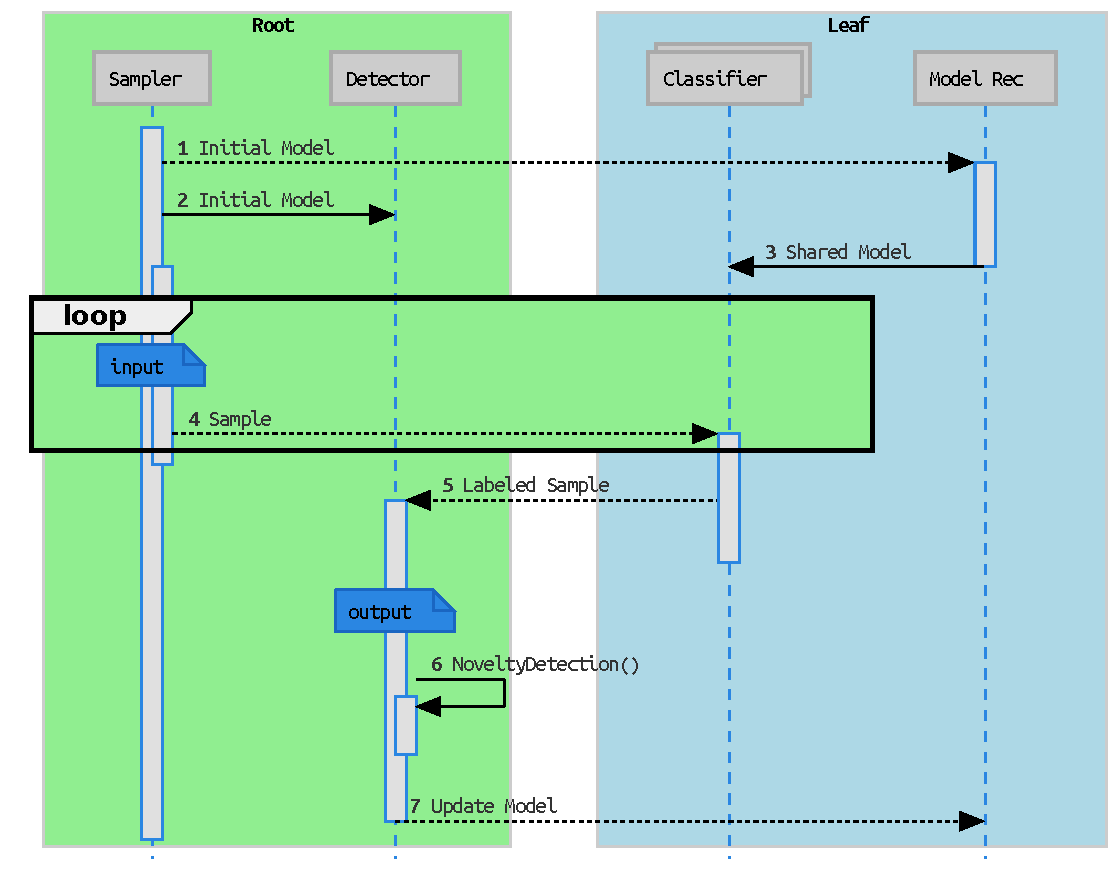
\includegraphics[width=0.75\linewidth,page=1]{figures/lifecycle-uml-svg.pdf}
  }
  \caption{\mfog life line overview.}
  \label{fig:mfog-mpi-life}
\end{figure}

% \FloatBarrier
% ------------------------------------------------------------------------------
\section{Metodologia de Avaliação}\label{sec:avaliacao}

% \nota{reestrutura 2:
%   A - cenario
%   B - metodologia (como, o que vai implementar [kafka, python, flink], como avaliar)
%   C - métricas (escalabilidade, qualidade)
%   D - resultados preliminares (python/kafka, flink)
% }

A avaliação da proposta aqui apresentada é feita por meio de métricas da
literatura, divididas em duas partes: métricas de qualidade de classificação
e métricas de escalabilidade.

As métricas de qualidade de classificação escolhidas devem ser adequadas para
avaliar detecção de novidades em fluxos de dados, felizmente o tratamento necessário é
estabelecido por \citeonline{Faria2013evaluation} e expandido por
\citeonline{DaSilva2018,DaSilva2018thesis,Costa2019,Costa2019thesis}.
Além do tratamento estabelecido, as métricas adaptadas não são calculadas
somente para o conjunto completo capturado no final do fluxo, e sim para cada
exemplo $\mathbf{X}$ classificado.
Portanto, as métricas têm como índice o contador de exemplos $x$, informando a
posição do exemplo em relação ao fluxo, ou seja, as métricas são de todos os
exemplos até a instância $x$.

\begin{definition}
  O problema de Detecção de Novidades em fluxo de dados pode ser modelado como
  uma função $f$ onde, dado o um exemplo $\mathbf{X}$ de um fluxo de dados $S$,
  pertencente a uma classe real $c \in \mathbf{C}$, é associado a um rótulo $l
  \in \mathbf{L}$ podendo ser uma classe conhecida $c' \in \mathbf{C}'$, ``desconhecido''
  ou um rótulo novidade $y \in \mathbf{Y}$:
  \begin{align}
    f  &: \mathbf{X} \mapsto l  \quad \mathbf{X} \in S , \quad l \in \mathbf{L}
      &&\text{Função de classificação} \label{eq:classifieFN} \\
    \mathbf{C} &= \{ c_1, c_2, \cdots, c_m \}
      &&\text{Classes do problema} \label{eq:classes} \\
    \mathbf{C}' &\in \mathbf{C}
      &&\text{Classes no treinamento} \label{eq:knownClasses} \\
    \mathbf{Y} &= \{ y_1, y_2, \cdots, y_k \}
      &&\text{Rótulos Novidade} \label{eq:novelies} \\
    \mathbf{L} &= \{ l_1, l_2, \cdots, l_n \} = \mathbf{C}' \cup \{ \text{``desconhecido''} \} \cup \mathbf{Y}
      &&\text{Rótulos Produzidos}\label{eq:labels} 
  \end{align}
\end{definition}

O tratamento estabelecido das métricas de qualidade para mineração de fluxos de dados define
que as métricas sejam extraídas de uma matriz de erro de classificação
multi-classe $\mathbf{E}_x$ na \refequ{matrix}, adaptada para detecção de
novidade.

\begin{definition}
  Uma matriz de confusão $\mathbf{E}$ para a instância $x$, de dimensão $m \times
  n$ para $m$ classes e $n$ rótulos, é preenchida com o número de instâncias da
  classe $c_i$ classificados com o rótulo $l_j$.
  \begin{align}
    \mathbf{E}_x = (e_{ij})\in \mathbb{N} ^{m\times n}
    &= \begin{pmatrix}
      e_{1,1} & e_{1,2} & \cdots & e_{1,n} \\
      e_{2,1} & e_{2,2} & \cdots & e_{2,n} \\
      \vdots  & \vdots  & \ddots & \vdots  \\
      e_{m,1} & e_{m,2} & \cdots & e_{m,n} 
    \end{pmatrix}  \label{eq:matrix}
  \end{align}
\end{definition}

Note que a soma de todos os elementos da matriz de confusão é igual a $x$, ou
seja, a contagem de todos exemplos.

Um dos possíveis rótulos $l_j \in \mathbf{L}$ é o rótulo ``desconhecido'', que
indica um erro de classificação diferente dos demais e é tratado separadamente.
A taxa de desconhecidos $\mathit{UnkR}$ na \refequ{unkr} é uma das métricas escolhidas
pois trata deste tipo específico de erro \cite{Faria2013evaluation}.

\begin{definition}
  A taxa de desconhecidos $\mathit{UnkR}_x$ (\refequ{unkr}) para um instante $x$ é definida como
  a média da taxa de desconhecidos de cada classe \cite{Faria2013evaluation}.
  % \begin{align}
  %   \mathit{UnkR}_x & = \frac{1}{m} \sum_{i=1}^{m} \mathit{UnkR}_{x, i}
  % \end{align}
  A taxa de desconhecidos de cada classe $c_i$ (\refequ{unkrXI}) é definida como o elemento
  $e_{ij} \in \mathbf{E}_x$ onde $j$ é a coluna do rótulo ``desconhecido''
  na matriz de rótulos $\mathbf{L}$ dividido pelo número de exemplos da classe.
  \begin{align}
    \mathit{UnkR}_{x, i}
      &= \frac{e_{i j} : l_j = \text{``desconhecido''}}{\sum_{j=1}^{n} e_{i j}}
      \label{eq:unkrXI}\\
    \mathit{UnkR}_x & = \frac{1}{m} \sum_{i=1}^{m} \mathit{UnkR}_{x, i}
    \label{eq:unkr}
  \end{align}
\end{definition}

Para todos os rótulos $l_j$ diferentes de ``desconhecido'', uma classe $c_i$ é
associada se o rótulo $l_j$ é procedente do modelo inicial, ou seja $l_j = c_i :
c_i \in \mathbf{C}'$ ou, em último caso, o rótulo $l_j$ é associado à classe com
o maior número de exemplos com o rótulo $l_j$, ou seja $e_{ij} = max\{ e_{aj} :
a \in [0, m] \}$ para $c_i \in \mathbf{C}$ e $l_j \in \mathbf{L}$
\cite{Faria2013evaluation}.
Estas regras de associação podem ser expressas pela função de associação vista
na Equação \ref{eq:assosiationFN}.

\begin{definition}
  A função de associações $A(l)$ é definida como:
  % $0$ se o rótulo é ``desconhecido'',
  % $i$ se o rótulo $l_j$ está no conjunto de classes $\mathbf{C}$,
  % $i$ se o rótulo $l_i$ está no conjunto de classes $\mathbf{C}$,
  \begin{align}
    A(l_j) : l_j \in \mathbf{L} \mapsto c_i \in \mathbf{C} &= \begin{cases} 
      \text{indefinido}        & \quad \text{se } l_j = \text{``desconhecido''} \\
      c_i         & \quad \text{se } \exists c_i = l_j \quad: c_i \in \mathbf{C}' \\
      c_i         & \quad \text{se } e_{ij} = max\{ e_{aj} : \in [0, m] \}
    \end{cases}
    \label{eq:assosiationFN}
  \end{align}
\end{definition}

No contexto de classificação multi-classe, a acurácia $\mathit{acc}_x$ para um
instante $x$ é definida como a média da acurácia de cada classe (\refequ{acc}).
A acurácia de cada classe $c_i$ no instante $x$, de forma semelhante à
definição da matriz de confusão, é definida como extensão da acurácia da
classificação binária (\refequ{acci}).
Para classificação binária a acurácia calculada com os valores
verdadeiro-positivo ($tp$), verdadeiro-negativo ($tn$), falso-positivo ($fp$) e
falso-negativo ($fn$).
Para cada classe $c_i$, o valor verdadeiro-positivo ($tp_i$) é definido como
número de exemplos onde o rótulo do exemplo $l$ é associado à
classe $c_i$ (\refequ{tpi}).
O valor falso-negativo ($fn_i$) são os exemplos da classe onde o
rótulo do exemplo não é associado à classe $c_i$ e o rótulo não é ``desconhecido'' (\refequ{fni}).
Os valores verdadeiro-negativo ($tn$) e falso-positivo ($fp$) são zero.
% pois dado um exemplo de classe $c_i$, ele pode ser classificado como .
% O como os valores $tp_i$ e $fp_i$ cobrem toda a matriz de confusão ($tp_i + fp_i = x$)

% \begin{definition}
%   A função de associações $A = (a_j) \in \mathbb{N}^n$ um item $a_j$ é
%   igual ao índice $i$ da classe $c_i$ associada ao rótulo $l_j$ sendo:
  \begin{align}
    tp_i            &= \sum_{j=1}^{n} e_{ij}        \quad \text{ se } l_j \neq \text{``desconhecido''} \text{ e } A(l_j) = c_i \label{eq:tpi}\\
    fn_i            &= \sum_{j=1}^{n} e_{ij}        \quad \text{ se } l_j \neq \text{``desconhecido''} \text{ e } A(l_j) \neq c_i \label{eq:fni}\\
    \mathit{acc}_i  &= \frac{tp + tn}{tp+fn+fp+tn}  = \frac{tp_i}{fn_i + tp_i} \label{eq:acci}\\
    \mathit{acc}_x & = \frac{1}{m} \sum_{i=1}^{m} \mathit{acc}_{i} \label{eq:acc}
  \end{align}
% \end{definition}

Concluindo as métricas de qualidade de classificação, a métrica de erro
combinado ($err$) é a média do erro de cada classe, sendo o erro de cada classe
o valor falso-negativo ($fn_i$) dividido pelo número de exemplos da classe.

\begin{align}
\mathit{err} &= \frac{1}{m} \sum_{i=1}^{m} \frac{fn_i}{fn_i + tp_i}
\end{align}

% \begin{definition}
%   A função de associações $A = (a_j) \in \mathbb{N}^n$ um item $a_j$ é
%   igual ao índice $i$ da classe $c_i$ associada ao rótulo $l_j$ sendo:
%   \begin{align}
%     FPR_i &= \frac{fp_i}{fp_i + tn_i}  & FNR_i = \frac{fn_i}{fn_i + tp_i} \\
%      \label{eq:cer}
%   \end{align}
% \end{definition}

% In the confusion matrix $M = m_{ij} \in \mathbb{N} ^{c \times{} l}$, computed by
% our evaluation script, each row denotes % one of the data sets original 
% the actual class $c$ and each column denotes the predicted label $l$ present in
% the captured output stream.
% Thus, each cell $M_{c, l}$ contains the count of examples from the test data set
% of class $c$ found in the output stream with the label $l$ assigned by the under
% evaluation experiment.

% Na matriz de confusão $\mathbf{E}_n$, a posição $e_{i,j}$

% As métricas de qualidade de classificação selecionadas para avaliar a
% implementação do \mfog são a 
% taxa de desconhecidos $UnkR_n$ na \refequ{unkr} \cite{Faria2013evaluation},
% acurácia média $acc_n$ na \refequ{acc}
% e Macro F-score ($Fscore$ na \refequ{fscore}, também referido na literatura por
% F1M) \cite{Sokolova2009,DaSilva2018thesis}.
% As métricas são extraídas para todos os exemplos classificados (instantes $n$)
% da respectiva matriz de erro $\mathbf{E}_n$.

% % \nota{'para todos os instantes n' ??}

% % \nota{Explicar o que significa cada elemento nas fórmulas}

% \begin{align}
%   \mathit{acc}_n        &= \frac{1}{M} \sum_{i=1}^{M} \frac{tp_i + tn_i}{tp_i+fn_i+fp_i+tn_i}
%   = \frac{1}{M} \sum_{i=1}^{M} \frac{\#Acc_i}{\#ExC_i}  \label{eq:acc} \\
%   \mathit{CER}_n        &= \frac{1}{M} \sum_{i=1}^{M} \frac{fp_i + fn_i}{tp_i+fn_i+fp_i+tn_i}
%   = \frac{1}{M} \sum_{i=1}^{M} \frac{\#Acc_i}{\#ExC_i}  \label{eq:cer} \\
%   \mathit{Precision}_n  &= \frac{1}{M} \sum_{i=1}^{M} \frac{tp_i}{tp_i+fp_i} \\
%   \mathit{Recall}_n     &= \frac{1}{M} \sum_{i=1}^{M} \frac{tp_i}{tp_i+fn_i} \\
%   \mathit{Fscore}\beta_n &= (\beta^2 +1) \cdot
%   \frac{
%   \mathit{Precision} \cdot \mathit{Recall}
%   }{
%     \beta^2 \cdot \mathit{Precision} +\mathit{Recall}
%   }\\
%   \mathit{Fscore}1_n   &= 2 \cdot \frac{
%     \mathit{Precision} \cdot \mathit{Recall}
%     }{
%       \mathit{Precision} +\mathit{Recall}
%     } \label{eq:fscore}
% \end{align}
% % = 2 \cdot \frac{tp}{2 \cdot tp + fn + fp}
% % \mathcal{L}         &= \frac{-1}{N} \sum_{i=1}^{M} \sum_{j=1}^{J} y_{i,j} \log(p_{i,j})

% % \nota{usar coeficiente d-intra vs d-extra grupo para determinar K de
% % cada label. Também pode-se usar os mesmos coeficientes para _log_}

% A transformação do fluxo de saída em uma matriz de erro é realizada no \sink,
% \notahl{como tratar o paralelismo desse elemento?\\
% Ele dá conta de todo o fluxo recebido dos classificadores?}
% \hlhl{onde} 
% \hlhl{tem-se disponível o fluxo original}
% \hlhl{com as rótulos corretas e o fluxo resultante}
% \hlhl{da classificação.}
% Esse módulo deve levar em consideração que pode haver reclassificação de um
% evento, previamente rotulado como desconhecido, em padrões oriundos de classe
% novidade ou extensão devido ao processo de detecção de novidades executado
% posteriormente ao surgimento do padrão em questão.

% Portanto os resultados são computados em função do fluxo de saída, então os $n$ nas
% equações são o índice do evento de saída.
% $\mathbf{unk}$ é o conjunto de eventos marcados como desconhecidos.
% \nota{oque eh unk? nesse paragrafo acima, erro de compilacao do latex?}

% \nota{frase confusa, eh so tirar o COMO e quebrar a frase: Esse módulo deve levar em consideração que
% COMO pode haver reclassificação de um evento, previamente rotulado como
% desconhecido, em padrões oriundos de classe novidade ou extensão devido ao
% processo de detecção de novidades executado posteriormente ao surgimento
% do padrão em questão}

% \begin{align}
%   E_{n,i,j} &= \bordermatrix{~ & c_i & \neg c_i \cr
%   l_j       & TP = \alpha           & FP = \gamma - \alpha                 \cr
%   \neg l_j  & FN = \beta - \alpha   & TN = n - (\alpha + \beta + \gamma)  \cr} \\
%   FM1       &= \frac{TP}{TP+\frac{FP+FN}{2}}
% \end{align}

% Os valores da matriz de erro para 

% \begin{align}
%   \alpha _j &= max( \{ |e_{i,j}|: i = 1 .. I \wedge \in \mathbf{E}_n \})
%           & \text{máximo da linha (rótulo)} \\
%   a_j &= i: |e_{i,j}| = \alpha _j
%           & \text{índice da classe associada à rótulo} \\
%   \beta   &= \sum_{j = 0}^{J} e_{i,j} : e_{i,j} \in \mathbf{E}_n
%           & \text{soma de uma coluna (rótulo)} \\
%   \gamma  &= \sum_{i = 0}^{I} a_{i,j} : e_{i,j} \in \mathbf{E}_n
%           & \text{soma de uma linha (classe)}
% \end{align}

Para a validação da corretude da implementação do \mfog com relação ao algoritmo
\minas original, ambos são executados com o mesmo \dataset de avaliação e as métricas de
qualidade de classificação são comparadas.

% As métricas de escalabilidade selecionadas são: número de nós processadores,
% tipo de processadores, uso de memória, tempo de processamento, taxa de eventos
% processados e latência entre a produção e classificação de um evento.

% \begin{align}
%   \Delta { } t_n       &= t_{n,sink} - t_{n,source} \label{eq:delta-t} \\
%   \overline{\Delta { } t}_n       &= \frac{1}{N} \sum_{i=1}^{N} \Delta { } t_n  \label{eq:avg-delta-t} \\
%   \alpha &= \# processors \\
%   \gamma &= \frac{\overline{\Delta { } t}}{}
% \end{align}

% \nota{
% como assim os resultados sao validos so se tiverem essas metricas? Entao quer
% dizer que qual medida eh valida? Vc quis dizer que se as medicoes que vc extrair
% com essas metricas forem iguais as medicoes do minas original, entao ai eh
% valido. Eh Isso?
% }

% Da implementação do \mfog é prevista a execução de experimentos com \datasets
% diversos, em especial os \datasets reais como \emph{Kyoto 2006+},
% que contenham evolução de conceitos.
% Os resultados desses experimentos irão conter as seguintes métricas:

% \begin{enumerate}[label={\alph*)}]
%   \item Qualidade de classificação (taxa de desconhecidos, acurácia e erro);
%   \item Escalabilidade (número de processadores, volume processado, tempo
%   decorrido);
%   \item Recursos computacionais utilizados (memória, tempo de processamento,
%   operações de leitura e escrita).
% \end{enumerate}

% ------------------------------------------------------------------------------
% Conclusão artigo

% We have used two types of evaluation measurements for each experiment:
% a measure of the full experiment execution time
% % extracted by using \emph{GNU Time 1.9} measuring 
% and, a set of qualitative measurements % será que é relevante falar da captura em Python?
% extracted by a Python script.

Um programa de avaliação foi construído seguindo as técnicas de referência como
matriz de confusão multi-classe com associação de classe de rótulo
\cite{Faria2016minas} para extrair medidas de qualidade de classificação.
Este programa recebe duas entradas, o conjunto de dados de teste e o fluxo de
saída capturado.
Com estas informações o programa gera a matriz de confusão do instante final, associação de
classes e rótulos, resumo de qualidade final com
\emph{Hits} (acurácia), \emph{Misses} (erro), \emph{Unknowns} (taxa de
desconhecidos) e, um gráfico de visualização do fluxo com as métricas e
marcadores de novidades para cada instante do fluxo de saída capturado.

As métricas de escalabilidade extraídas são o número de processadores, tempo de
processamento e latência de eventos e, estas métricas permitem o cálculo de
\emph{speedup} prático.

% % Our script computed the
% Our evaluation script was build following reference techniques like
% multi-class confusion matrix with label-class association \cite{Faria2016minas}
% to extract classification quality measurements.
% This script takes two inputs, the test data set and the captured output stream,
% and outputs the confusion matrix, label-class association,
% final quality summary with:
% \emph{Hits} (true positive), \emph{Misses} (Err), \emph{Unknowns} (UnkR); and
% stream visualization chart with per example instance summary with novelty label markers.
% % 
% % For clarity, it is necessary to detail how to interpret and compare each measure,
% % as for some it is trivial but others are not so much.

% In the confusion matrix $M = m_{ij} \in \mathbb{N} ^{c \times{} l}$, computed by
% our evaluation script, each row denotes % one of the data sets original 
% the actual class $c$ and each column denotes the predicted label $l$ present in
% the captured output stream.
% Thus, each cell $M_{c, l}$ contains the count of examples from the test data set
% of class $c$ found in the output stream with the label $l$ assigned by the under
% evaluation experiment.

% For the data set under use, original classes are $c \in \{N, A\}$, and for the
% labels we have the training class
% \emph{``N''}, \emph{unknown} label \emph{``-''} and the novelties $i \in
% \mathbb{N}$ so $l \in \{N, -\} \cup \mathbb{N}$.

% Added to the original confusion matrix $M$ are the rows \emph{Assigned} and
% \emph{Hits}.
% \emph{Assigned} row represents which original class $c$ (or if \emph{unknown},
% \emph{``-''}) the label $l$ is assigned to, this is computed by using the
% original class if $c = l$ or by associated novelty label to original class as
% described in \cite{DeFaria2015evaluation} section 4.1
% (class from where the most samples came from).
% \emph{Hits} row shows the true positive count for each label $l$
% with assigned class $c$, being the same value as cell $M_{c, l}$.
% % computed by coping the value of the 
% %  where the label is the same
% % and the class $c$ is the value in the above \emph{Assigned} row.
% The \emph{Hits} row is also used to compute the overall true positive
% in the summary table and stream visualization chart.
% % accuracy.
% One complete matrix is shown in Tab. \ref{tab:java-matrix}.


% \section{Descrição da Arquitetura Proposta}\label{sec:descricao}

% \newcommand{\source}{módulo auxiliar \emph{source}\xspace}
% \newcommand{\sink}{módulo auxiliar \emph{sink}\xspace}

% \newcommand{\offline}{módulo treinamento\xspace}
% \newcommand{\classify}{módulo classificador\xspace}
% \newcommand{\detector}{módulo detector de novidades\xspace}

% Nesta Seção, apresenta-se o \mfog, objeto proposta deste trabalho.
% O \mfog é composto de três módulos principais e dois auxiliares.
% Os módulos principais implementam o algoritmo MINAS, sendo eles: \offline
% (\emph{Training Module}), \classify (\emph{Classification Module}) e
% \detector (\emph{Novelty Detection Module}).
% Dois módulos auxiliares são utilizados para avaliação do \mfog:
% \source (fonte) e \sink (sorvedouro, consumidor final).
% Os módulos e as interações entre eles são ilustradas na \reffig{arch}.

% \begin{figure}[ht]
% \centering
% 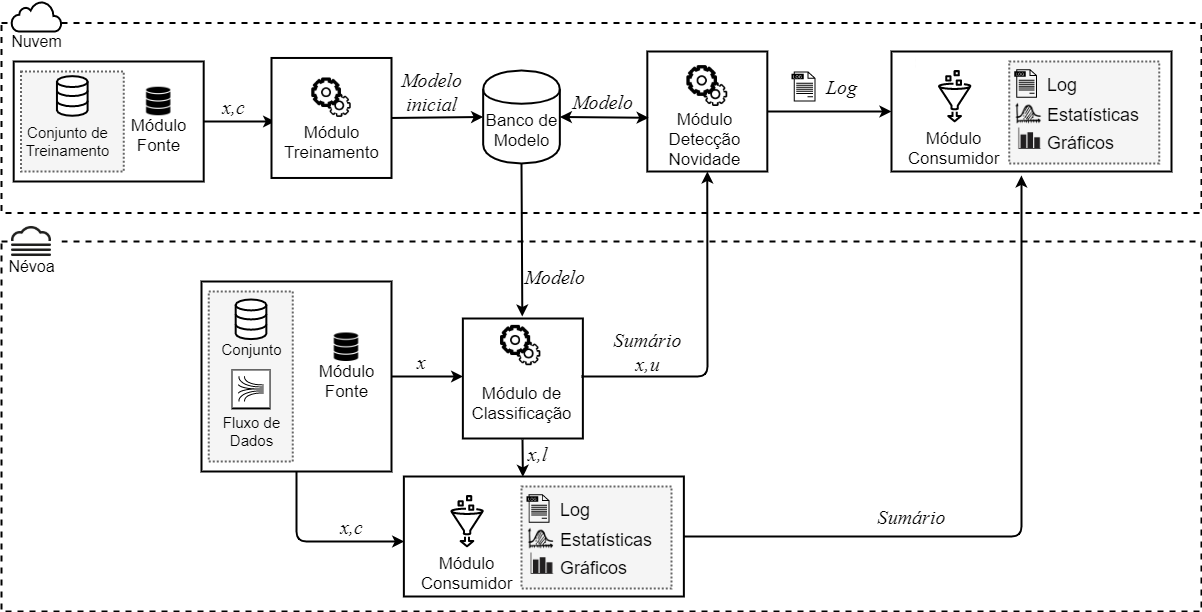
\includegraphics[width=\textwidth]{figuras/mfog-arch-v3_pt-br.png}
% \caption{Arquitetura e fluxos de dados do \mfog.}
% \label{fig:arch}
% \end{figure}

% A implementação do \mfog segue a arquitetura \arch formalizada por
% \citeonline{Cassales2019a}, discutida na \refsec{cassales}.
% A arquitetura \arch
% % (e outras arquiteturas de NIDS)
% estabelece que um serviço de
% captura e tratamento de dados é instalado na borda de uma rede local com
% dispositivos \iot.
% Na presente implementação, esse serviço de captura e tratamento é representado
% pelo \source.

% O \source é dependente da fonte de dados, executando a transformação dos
% formatos dos \datasets para um fluxo de exemplos (representado por $x$ na \reffig{arch})
% compatível com o restante da implementação.
% Além de fornecer exemplos tratados para o \classify, o \source também fornece
% exemplos com a classe original (representado por $x,c$ na \reffig{arch})
% \notafa{somente na fase de treinamento o source fornece exemplos rotulados par ao sink, certo?}
% \hlfa{para o \sink e para o \offline}.

% O \sink é responsável por agregar todos resultados do \mfog e,
% juntamente com os valores do \dataset fornecidos pelo \source, por computar
% as métricas de qualidade de classificação.
% Além disso, esse módulo também coleta e agrega métricas base para as avaliação de
% escalabilidade e métricas de uso de recursos computacionais.

% Os dados resultantes do serviço de captura e tratamento (representado no \mfog
% pelo \source) são ingeridos pela aplicação no \classify. A ingestão é feita por
% meio de um operador fonte, fornecida pela plataforma \flink.
% % \notake{TCP e apache flink}
% % conexão TCP (\emph{Transmission Control Protocol}).
% Na plataforma, com o modelo de classificação disponível, os exemplos são
% classificados seguindo o algoritmo MINAS original discutido na \refsec{minas-og}.
% A rótulo atribuída pela classificação, ou meta-rótulo de desconhecido,
% juntamente com o exemplo original (representado por $x,l$ na \reffig{arch})
% são enviados para o \sink.
% Além disso, se o exemplo não for classificado, o exemplo e a meta-rótulo de
% desconhecido (representado por $x,u$ na \reffig{arch}) são enviados para o
% \detector.
% \notahl{processaa ND em paralelo?}
% Outra comunicação é o envio das modificações ao sumário estatístico do modelo de
% classificação (representado por $Summary$ na \reffig{arch}) do \classify para o
% \detector.

% O \detector é responsável por executar o processo de detecção de novidade,
% atualizando o modelo de classificação, e entregar o novo modelo às instâncias do
% \classify, através do serviço de armazenamento de modelo (\emph{Model Store} na
% \reffig{arch}).
% O \detector também envia meta-informações sobre o processo de detecção de
% novidade (representado por $Log$ na \reffig{arch}) para o \sink.

% \nota{
% nao seria legal fazer um diagrama pq ai vc pode usar ate nos slides de como eh
% essa implementacao. Faz no draw io pra que de pra usar na monografia e de para
% enxergar na apresentacao
% }

% flink ainda... revisar...

% O \mfog utiliza em seus módulos a distribuição oferecida pela plataforma \flink
% como paralelização, ou seja, utiliza uma instância de trabalho (\emph{job}) por
% dispositivo de classificação, sendo que cada instância de trabalho aloca um
% gerenciador de tarefas por processador.
% Dessa forma, busca-se a escalabilidade no ambiente de \fog para o \classify.
% O \offline, por ser utilizado somente uma vez para gerar o modelo
% de classificação inicial, não tem impacto na escalabilidade geral do sistema.
% O \detector também é implementado na plataforma \flink e, por ser hospedado em
% ambiente de \cloud, herda as qualidades desse ambiente incluindo escalabilidade.
% \notake{destaque sentença}
% O restante do sistema (\source, \sink, armazenamento de modelo) não é foco deste
% estudo e sua escalabilidade, desde que não afete a escalabilidade do \classify e
% \detector.
% \notahl{Questões que precisam ser tratadas:\\
% - Paralelização da classificação: como agrupar os dados e dividir o processamento?\\
% - ND: como saber o que agrupar (dos nós) e como dividir?
% Padrões podem ser locais? Ou sempre se aplicam a todos os nós?}
% \notafa{frase incompleta}
